% intervals (for ISPASS'03)
%
\documentclass[10pt,dvips]{article}
%\documentclass[10pt,twocolumn,dvips]{article}
\usepackage[english]{babel}
\usepackage{epsfig}
%\usepackage{fancyheadings}
%\usepackage[T1]{fontenc}
%\usepackage[latin1]{inputenc}
%\usepackage{twocolumn}
%\usepackage{verbatim,moreverb,doublespace}
%\usepackage{rotate,lscape,dcolumn,array,rotating,latexsym}
%
%\input{epsf}
%
% for somebody (I forget now !)
%\textwidth 175mm
%\textheight 225mm
%\topmargin -4.5mm
%
% for somebody else (I also forget now !)
%\textwidth 6.6in 
%\textheight 239mm
%\topmargin -15mm
%\leftmargin -2.0in
%
% for (IEEE single-column format)
%\textwidth 6.875in
%\textheight 8.875in
%\topmargin -0.6in
%\oddsidemargin 0mm
%\evensidemargin 0mm
%
% for HPCA (IEEE two-column format)
%\textwidth 6.5in
%\textheight 8.875in
%\topmargin -0.4in
%\oddsidemargin 0mm
%\evensidemargin 0mm
%
% for ISPASS
\textwidth 6.5in
\textheight 8.875in
\topmargin -0.4in
\oddsidemargin 0mm
\evensidemargin 0mm
%
%
% turn the following (linespread) on to 1.6 for "double space"
\linespread{1.6}
%
%
% some publishers want no page numbers for final print
%\pagestyle{empty}
%
\begin{document}
%
%
%
\title{Implications of Register and Memory Temporal Locality for
Distributed Microarchitectures}
%
%
\author{
A. Khalafi, D. Morano, D.R. Kaeli\\
Northeastern University\\
{akhalafi, dmorano, kaeli}@ece.neu.edu\\
\and
A.K. Uht\\
University of Rhode Island\\ 
uht@ele.uri.edu
}
%
%
% some publishers do not want a data in the final print
\date{}
%
\maketitle
%
% uncomment the following for page with no page numbers (for IEEE)
%\thispagestyle{empty}
%
%
\begin{abstract}
%
We explore various intervals between register
assignments and the subsequent uses of the same registers.
We also explore memory stores and the
subsequent loads to the same memory addresses.
Three different types of access intervals
are defined and data are gathered on them using benchmarks.
This data serves to provide insight
about how a suitable microarchitecture might take advantage
of the register or memory access behavior in order to reduce the overhead
of accessing centralized machine resources like
a register file (in the case of register operations)
or the general memory hierarchy in the case of memory
operations.
A proposed distributed microarchitecture is briefly presented
and data about its ability to allow operand bypassing
of centralized machine resources
to satisfy memory load requests is provided.
%
\end{abstract}
%
%
%\vspace{-0.25in}
\section{Introduction}
%\vspace{-0.15in}
%
As computer microarchitectures have increased in complexity and
size, the need to access and update centralized microarchitectural
resources has become increasing problematic.
Access contention for centralized microarchitectural resources
increases substantially as the machine is enhanced to perform
a greater and greater number of operations in parallel.
The goal of these microarchitectures is to generally increase
program execution performance through the extraction of higher
amounts of Instruction Level Parallelism (ILP) from substantially
sequential programs.
Generally, this is achieved by introducing multiple
execution units into the microarchitecture where each unit
can independently process a part of the single threaded program's
instruction stream.  
However, these multiple execution units
still all need access to a common set of architected machine registers
as well as the architected memory of the computer.
In addition to access contention for centralized resources,
the routing complexity required to access and update those
resources becomes an increasingly difficult implementation issue
in the silicon layout.

Some example microarchitectures that have explored the
use of multiple execution units are the Multiscalar-like
processors ~\cite{Sohi95,sundararaman97multiscalar},
the SuperThreaded processor model ~\cite{tsai96superthread},
and
the Parallel Execution Window processor model ~\cite{kemp96pew}.
Other microarchitecture proposals such as the MultiCluster machine
model by 
Farkas et al ~\cite{farkas97multicluster} are also in this category.
More recently, much work on trace processor microarchitecture 
models ~\cite{rotenberg97trace,vajapeyam97sequences,rotenberg99control}
have also explored multiple distributed execution units and their associated
problems.
Another example of a distributed microarchitecture is that
of the Grid Processor described by Nagarajan et al ~\cite{Nag01}.
Further, microarchitectures have been proposed that feature both
large numbers of distributed execution units along with more
generalized multipath execution ~\cite{uht02realizing,morano02high}.
These are also keenly sensitive to the problems associated with accessing
centralized machine resources.

In addition to these research oriented microarchitectures, it should
be noted that processors such as the 
Silicon Graphics (SGI) R10000 ~\cite{yeager96r10000}, 
and the Digital Equipment (DEC) processor such as the
Alpha 21264 ~\cite{leibholz97alpha,Kessler98}
also feature multiple execution units.
Although these latter processors are not generally considered to
feature large distributed microarchitectures, they represent a 
possible trend as to where commercial microarchitectures might evolve.
As the number of execution units in the microarchitecture increases
beyond eight, sixteen or more, there will be an increasing need
to consider the problems associated with accessing both
the memory hierarchy as well as even the architected register
file.
%% NOTE citation for EV8

The more obvious examples of centralized machine resources include
the register file (for register access and update),
and the L1 data cache for memory location access and update.
Other machine resources also form bottlenecks to increasing
execution parallelism but those are not the focus of this present
paper.
In the case of memory, there is a further dimension associated
with it beyond the problems of access and update contention.
The additional problem for memory access is the long latencies
that can be incurred especially for memory reads.
While the currently used general memory hierarchy
attempts to substantially solve
the problem associated with long access latencies, the problem of
handling many accesses simultaneously due to machine parallelism remains.
An example of a microarchitecture mechanism to better handle
multiple simultaneous memory requests was the Address Resolution
Buffer by Franklin and Sohi ~\cite{franklin96arb}.
An example of providing distributed access to the architected
register file is that described by Jiser et al with their
\textit{Global Register Partitioning} ~\cite{Jiser00}.
However, their approach (and similar to that of the Multiscalar
work and the Grid Processor work mentioned above) includes
the use of the compiler to facilitate a total distributed 
machine model.
We are interested in a more restricted design space where an existing
ISA must be maintained such as the case with the R10000 or the Alpha
processors.

Our primary goal is the investigation of distributed microarchitectures
(similar to many of the above examples) that feature very large
instruction windows with multiple distributed execution units.
We want to explore the feasibility of having in-flight operands
(of both register or memory variety) bypass both the
architected register file as well the traditional L1
data cache and the load-store queue (LSQ) for subsequent uses of
those operands.
Although the register operand bypassing of the architected register 
file has been done for a long time ~\cite{Tom67},
it has not been expanded into the realm of large and spatially distributed
microarchitectures.
Also, as the snooping of the familiar load-store queue can be
thought of as bypassing (if there is a hit) the L1 data cache, it
itself simply becomes the next centralized resource for which
access contention becomes the problem.
We want to investigate the feasibility of having 
either register or memory operands bypass any centralized
machine resource entirely.  
Two general mechanisms can be envisioned to facilitate
operand bypass.  
One such mechanism is the direct forwarding of a generated
operand from the source instruction to the corresponding sink
instructions.
This can generally only occur when
both the source of the operand and the instruction sinks of the same
operand are both located within the instruction window of the
processor at the same time.  
This prompts the question as to how
often this can be expected to occur.
The second general mechanism to facilitate operand
bypass is the use of buffering or caching within the execution
window of the processor.
More specifically, this would constitute either buffering or caching of
operands at some spatial location between operand sourcing instructions
and the corresponding sink instructions for the same operands.

This paper explores the access intervals, as measured in dynamic 
instructions executed, between assignment to
registers and their corresponding uses, as well as the
assignment to memory locations (denoted by a memory address) and their 
corresponding uses.
We define three types of access intervals that we want to explore.
These access intervals are defined similarly for both register 
operations and
memory operations.
We have gathered data associated with each of our three access
intervals, for both register and memory operations, 
through the execution of general purpose sequential
program codes.
This work was substantially inspired by the prior work 
of Franklin et al ~\cite{Franklin92}
in their investigation of register traffic
for use in the context of the Multiscalar-like microarchitectures.
Prior work on memory locality has been substantial including
such work as Madison et al ~\cite{madison76characteristics},
Verkamo et al ~\cite{verkamo85emperical}, and more recently
that of Phalke et al ~\cite{phalke95gap} with their Inter-Reference
Gap work.
The present work builds on and extends that of Franklin et al
by providing
additional information on register operand traffic that was not
previously investigated.
We also extend the previous work of both Franklin et al and 
Phalke et al by applying our same measurements for register traffic
operations to memory traffic operations.

The rest of this paper is organized as follows.
Section 2 presents our definitions of the access intervals that
we studied along with some significance of those intervals
for microarchitectural design
decisions.
Section 3 presents our characterization results.
The results are presented in two parts.  
First for the register
operations and then for memory operations.
Section 4 presents an application that takes advantage
of operand bypass of centralized machine resources for both registers 
and memory.
The application consists of a proposed distributed microarchitecture,
briefly described,
that employs techniques to facilitate operand bypass.
Results on the effectiveness of operand bypass are given.
Section 5 summarizes the present work.
%
%\vspace{-0.25in}
\section{Definitions and Significance of Intervals}
%\vspace{-0.15in}
%
There are several possible intervals that can be defined with
regard to writes to a variable (whether a register or a memory
location) and the corresponding reads of the same variable.
We only explore three of these in this present work since
other possible intervals do not have as important significance
as the three types of intervals that we have selected.
We first provide some definitions for the intervals that
we have explored and then give some possible significance
to those intervals for microarchitectural design purposes.
%
%\vspace{-0.25in}
\subsection{Definitions of Intervals}
%\vspace{-0.15in}
%
We define all intervals in terms of the definition
(hereafter referred to as a \textit{def}) of a
\textit{variable instance} 
and the corresponding subsequent \textit{use} of the
same instance of the variable.
A write to any variable always constitutes a def of a new
variable instance.
A read to a variable constitutes a use of the associated
variable instance.
For our purposes, reads and writes occur on variables while
defs and uses occur for variable instances.
Variable instances are uniquely identified by both their variable 
address and their associated def (as identified in dynamic program
ordered time).
For registers, the address is generally just its name.  
For memory variables, the address is that of the memory
location itself.  
As alluded to already, a write to a variable 
destroys the previous instance of the variable while simultaneously
creating a new instance of that variable.  
This idea of variable instance is the same as that of 
Franklin et al ~\cite{Franklin92}.
A write to a variable is also assumed to constitute a def of a new
variable instance even if the
value assigned to the variable is the same as that which it
had already.
Uses of variable instances occur when the associated variable
is read for any architected reason, whether this is explicit
or implicit to the execution of an instruction.

We explore the following three types of access intervals on
both registers and memory locations :
%
\begin{itemize}
\vspace{-0.1in}
\item \textit{access-use}
\vspace{-0.1in}
\item \textit{useful-lifetime} (or \textit{def-last-use})
\vspace{-0.1in}
\item \textit{def-use}
\vspace{-0.1in}
\end{itemize}
%
The \textit{access-use} interval is defined as the number of
dynamic instructions from a read of a variable to the closest
of a preceding read or write to the same variable.
An access-use interval is therefor a property of a read of a variable.
Note that there may be many uses of the same instance of a variable.
Each read of a variable will therefor
usually have a different access-use interval associated with it
since the number of dynamic instructions from the def
of the variable instance to the current use is usually different.
Two uses may have the same access-use interval when,
for example, each is associated with an input operand to a single
instruction.
Our definition for the access-use interval is the same as the
\textit{inter-reference gap} from the work of 
Phalke et al ~\cite{phalke95gap}.
Franklin et al ~\cite{Franklin92} did not consider this type
of access interval in their work.

The \textit{useful-lifetime} is defined as the number of
dynamic instructions between the write of a variable
and the \textit{last} read of the same variable before the
subsequent write to the same variable.
This interval is also sometimes referred to as the \textit{def-last-use}
interval since only the last use of the variable instance is taken
into account when determining this interval.
This interval is therefor a property of the write to a variable.
Each write of a variable therefor only has one
useful-lifetime interval associated with it.
If there are, for example, three uses following the
def of a variable instance, only the last such use is
used to determine the useful-lifetime of the variable instance.
Note that the use-lifetime of a variable instance can have a value of 
zero.
The term \textit{useful-lifetime} is taken from Franklin ~\cite{Franklin92}.
This term is generally synonymous with the \textit{liveness} of
a variable instance ~\cite{hennpatt95}.
It should be noted that the term \textit{lifetime} is often confused
with that of useful-lifetime.
For our purposes, we define the term lifetime to refer to
the interval from a def of a variable instance (write to a variable)
to the
subsequent write of the same variable (thus creating a new
variable instance).
This is generally different than the def-last-use interval
for the same variable instance.
This definition of lifetime is the same as that used previously by
Franklin et al ~\cite{Franklin92}.
We do not further explore lifetime intervals in this
present work.

Finally, the \textit{def-use} interval is the number of
dynamic
instructions from the read of a variable to the preceding write
of the same variable.
As the case was with the access-use interval,
the def-use interval is a property of a read of a variable
and each such read will generally have a 
different def-use interval associated with it.
The exception occurs when two reads of the same variable occur in 
the same instruction (the
same as was the case with the access-use interval above).
Our definition for the def-use interval is also referred to
as the variable instance \textit{age} in the work by 
Franklin et al ~\cite{Franklin92}.
The idea of age is apparent since each use of a variable instance
can be thought of occurring at a certain age of the instance as
measured by the dynamic number of instructions since the associated
definition of the same instance.

A simple, and quite contrived, 
code example to illustrate the meaning of the three
intervals that we have defined is shown in Figure \ref{tab:code1}.
%
\begin{table}
\begin{center}
\caption{{\em Simple code example illustrating the different types of
access intervals.}
Alongside the instructions are the particular events generated
from those instructions and any intervals that can be calculated
as a result.}
\label{tab:code1}
\vspace{+0.1in}
\begin{tabular}{l|l|l|l}
\hline 
label&instruction&event&intervals determined\\
\hline 
\hline 
I1&\verb"r1 <= c"&def(r1)& \\
\hline
I2&\verb"r2 <= c"&def(r2)& \\
\hline
I3&\verb"r1 <= r2 + c"&def(r1), use(r2)&
access-use(r2)=1, def-use(r2)=1, useful-lifetime(r1)=0\\
\hline
I4&\verb"r2 <= r1 + c"&def(r2), use(r1)&
access-use(r1)=1, def-use(r1)=1, useful-lifetime(r2)=1\\
\hline
I5&\verb"r3 <= r1 + r2"&def(r3), use(r1),&
access-use(r1)=1, access-use(r2)=1,\\
 & &use(r2)&def-use(r1)=2, def-use(r2)=1\\
\hline
\end{tabular}
\end{center}
\end{table}
%
In this simple code example, the term \textit{c} is an arbitrary
immediate constant encoded within the instruction which is
also generally different for each instruction.
All of the instructions produce defs of a variable instance
associated with their destination registers.
Instructions I3 and I4 also produce uses of the registers \textit{r2}
and \textit{r1} respectively.
The def of register \textit{r1} in instruction I3 allows for the
determination of the useful-lifetime for the previous variable
instance (from instruction I1) held in that register.  
In the present example, the useful-lifetime for that
variable instance is calculated as 0.
This result is due to the fact there there were no intervening uses
of the register between instructions I1 and I3.
Likewise, register \textit{r2} is defed in instruction I4 and this
allows for the determination of the useful-lifetime for the previous
variable instance held in that register (from I2).  
That is calculated as being
being 1 since there was a use of that previous variable instance in
instruction I3.
Note that useful-lifetimes for a variable instance
cannot be determined until a subsequent
write of the corresponding variable is encountered.
Similarly, both instructions I3 and I4 contribute a def-use interval
with the value 1 since each represents a use of the corresponding
variable instance just one instruction after its associated def.
Finally from instruction I5, since there are uses of both registers
\textit{r1} and \textit{r2}, an access-use and def-use interval
can be determined for each of these.
Note that for register \textit{r1} an access-use interval with value
1 is determined while a def-use interval of value 2 is determined.
For register \textit{r2}, both its access-use and def-use intervals
have value 1 since there was a def of that register in just
the previous instruction.

Note that an access-use interval and a def-use interval is always 
determined for each
use of a variable instance, but that a useful-lifetime interval can
only be determined on a def of a new variable instance.
Although this example illustrated the determination of
the three types of access intervals on registers, these are
determined similarly for memory references.
%
%\vspace{-0.25in}
\subsection{Microarchitectural Significance of the Intervals}
%\vspace{-0.15in}
%
Each type of variable access interval that we are exploring
may have different significance or consequence 
for making microarchitectural design decisions.
Although all of the intervals discussed previously share
similar attributes, they tend to answer different microarchitectural
questions.
Firstly some types of intervals are associated with reads
while others are associated with writes.
This distinction is used when considering the applicability of each
type of interval metric.

The useful-lifetime interval is a property of a write
so data on these intervals would be useful when exploring
the desired microarchitectural consequences of a write occurring.
If, for example, the resulting operand from a write operation
could be buffered locally near the execution units in the processor,
on the average it would only have to remain buffered until
a number of following instructions (in dynamic program order)
equal to its
useful-lifetime had an opportunity to snoop the buffer for the
operand.
After the appropriate number of subsequent instructions had an 
opportunity to snoop the buffer, it could be assumed that
the likelihood of a further use of that operand is minimal
and therefor the operand could be released or evicted from the
buffer.

In contrast, since both the access-use interval and the def-use
interval is a property of a read, microarchitectural decisions
about how to best satisfy read operands might use the data associated
with either of these types of access intervals.
If we first consider the case of no intervening buffering or caching
of operands between an operand sourcing instruction and its
associated sink instructions, then the def-use interval data would
be appropriate to use for possible design decisions.
This is so because operand sinking type instructions could only
be satisfied by either a previous operand sourcing instruction
(allowing for operand bypass) or lacking that, the operand would have to be
fetched from the appropriate centralized resource (architected
register or future file in the case of a register, and the L1 data
cache or load-store queue in the case of a memory operand).

For those distributed microarchitectures that can employ
some sort of operand buffering or caching spatially close to
the execution units, the access-use interval is the more appropriate
metric to determine design decisions.
This is so because a cache of some sort can retain a copy of the
desired operand even though the original generation (original write)
of the operand may have occurred in the far past of the instruction stream.
Either the cache could maintain the operand for a reasonably long
period of time from a preceding write, or perhaps more likely, 
intervening reads keep
the cache from evicting the operand 
needed by possible subsequent sink instructions.
Further, a previous read could have resulted in the operand getting
cached from the appropriate centralized resource without even a near-past
write of the operand having ever occurred.
An example of a distributed microarchitecture that uses interspersed
caching of operands among the execution units is presented in Section 4.
%
%\vspace{-0.25in}
\section{Benchmark Statistics}
%\vspace{-0.15in}
%
In this section we present the results of accumulating our
access interval data on ten benchmark programs.
The programs are taken from the SpecINT-95 and SpecINT-2000
suites.
The following programs were used from SpecINT-95: GO, COMPRESS,
IJPEG.  
The following programs were used from SpecINT-2000:
BZIP2, CRAFTY, GCC, GZIP, MCF, PARSER, and VORTEX.
All programs were primarily compiled for the MIPS-1 ISA,
with a few MIPS-2 and MIPS-3 instructions included as a
consequence of executing any system library code.
The Silicon Graphics (SGI) vendor compiler was used for
all compilations under the Irix 6.4 operating system.
The programs were optimized using the '-O' compilation flag.
All programs were executed for 600 million instructions but
data was only collected and processed after skipping the
first 100 million.

The next subsection presents the results for register access use.
The following subsection presents the results for the memory 
access use.  For both registers and memory, data is shown for 
access-use, def-last-use (useful lifetime), and def-use
intervals.
%
%
%\vspace{-0.25in}
\subsection{Register Access Interval Results}
%\vspace{-0.15in}
%
In this section, we show the register access interval results for
our ten benchmark programs.
Figure \ref{fig:a_over} shows (top to bottom)
the three types of access intervals:
access-use, useful-lifetime, and def-use.
For each type of access interval, the data for each of the
ten benchmark programs are overlaid on the same graph.
For each access interval type, both a density 
and a distribution is provided.
%
\begin{figure}[tb]
\centering
\epsfig{file=a_over.eps,width=6.5in}
\caption{{\em Register Access Intervals.} 
Data results for all programs are shown overlaid.
The density is shown on the left and the distribution is shown
on the right.
All intervals are measured in dynamic numbers of executed instructions.}
\label{fig:a_over}
\end{figure}
%
As can be seen from the graphs of Figure \ref{fig:a_over},
all of the benchmark programs perform similarly and have
rather short (40 or less) interval lengths for most of each type
of access interval.
%
%
%\vspace{-0.25in}
\subsection{Memory Access Interval Results}
%\vspace{-0.15in}
%
In this section, we show the memory access interval results for
each of same benchmark programs as were used for the register interval
results.
The data are presented in three sets.
The first set of data is for register access-use intervals.
The second set of data is for register useful-lifetimes, and
the third is for register def-use intervals.

% MRINT
%
The data for memory access-use intervals are
shown in Figures \ref{fig:aa_mrint} 
and \ref{fig:ab_mrint}.
Results from benchmark programs BZIP2, COMPRESS, CRAFTY, GCC, and GO
are shown in Figure \ref{fig:aa_mrint} while the results
from programs GZIP, IJPEG, MCF, PARSER, and VORTEX are shown in
Figure \ref{fig:ab_mrint}.
%
\begin{figure}
\centering
\epsfig{file=aa_mrint.eps,width=6.0in}
\caption{{\em Memory Access-Use Intervals.} 
Data results for the 
BZIP2, COMPRESS, CRAFTY, GCC, and GO programs are shown.
The density is shown on the left and the distribution is shown
on the right.
All intervals are measured in dynamic numbers of executed instructions.}
\label{fig:aa_mrint}
\end{figure}
%
\begin{figure}
\centering
\epsfig{file=ab_mrint.eps,width=6.0in}
\caption{{\em Memory Access-Use Intervals.} 
Data results for the
GZIP, IJPEG, MCF, PARSER, and VORTEX programs are shown.
The density is shown on the left and the distribution is shown
on the right.
All intervals are measured in dynamic numbers of executed instructions.}
\label{fig:ab_mrint}
\end{figure}
%
%
% MLIFE
%
The data for memory def-last-use (or useful-lifetime) intervals are
shown in Figures \ref{fig:aa_mlife} 
and \ref{fig:ab_mlife}.
%
\begin{figure}
\centering
\epsfig{file=aa_mlife.eps,width=6.0in}
\caption{{\em Memory Def-Last-Use Intervals.} 
Data results for the 
BZIP2, COMPRESS, CRAFTY, GCC, and GO programs are shown.
The density is shown on the left and the distribution is shown
on the right.
All intervals are measured in dynamic numbers of executed instructions.}
\label{fig:aa_mlife}
\end{figure}
%
\begin{figure}
\centering
\epsfig{file=ab_mlife.eps,width=6.0in}
\caption{{\em Memory Def-Last-Use Intervals.} 
Data results for the
GZIP, IJPEG, MCF, PARSER, and VORTEX programs are shown.
The density is shown on the left and the distribution is shown
on the right.
All intervals are measured in dynamic numbers of executed instructions.}
\label{fig:ab_mlife}
\end{figure}
%
%
% MUSE
%
The data for register def-use intervals are
shown in Figures \ref{fig:aa_muse} 
and \ref{fig:ab_muse}.
%
\begin{figure}
\centering
\epsfig{file=aa_muse.eps,width=6.0in}
\caption{{\em Memory Def-Use Intervals.} 
Data results for the 
BZIP2, COMPRESS, CRAFTY, GCC, and GO programs are shown.
The density is shown on the left and the distribution is shown
on the right.
All intervals are measured in dynamic numbers of executed instructions.}
\label{fig:aa_muse}
\end{figure}
%
\begin{figure}
\centering
\epsfig{file=ab_muse.eps,width=6.0in}
\caption{{\em Memory Def-Use Intervals.} 
Data results for the
GZIP, IJPEG, MCF, PARSER, and VORTEX programs are shown.
The density is shown on the left and the distribution is shown
on the right.
All intervals are measured in dynamic numbers of executed instructions.}
\label{fig:ab_muse}
\end{figure}
%
%
In Figure \ref{fig:a_mcum} we show the cumulative data over all
benchmark programs.  That figure shows all three of the access
intervals that we explored: access-use, useful-lifetime, and def-use.
%
\begin{figure}[tb]
\centering
\epsfig{file=a_mcum.eps,width=6.0in}
\caption{{\em Cumulative Memory Intervals over all benchmarks.} 
The density is shown on the left and the distribution is shown
on the right.
All intervals are measured in dynamic numbers of executed instructions.}
\label{fig:a_mcum}
\end{figure}
%
As can be seen from the various figures for the memory access
intervals, unlike for the register intervals, these are significantly
varied from one benchmark program to another.
The more prominent spikes in several of the density graphs
is evidence of high frequency looping over memory.
It is interesting to note that GCC (and to a lesser extent GO)
has some pronounced
looping behavior for its access-use intervals but not for
its useful-lifetimes nor def-use intervals.
This represents more repeated reading of constant memory variables
rather than the more varied read-write memory behavior of 
most of the other programs.  Also, it is interesting to note
that most programs exhibit rather large useful-lifetimes of 0.
A zero-length useful lifetime represents a memory location that
is later overwritten without an intervening read.  
This
can happen when writing to output file buffers, for example, but can also
be due to control flow changes that abandon written variables.
The zero-length useful-lifetimes vary from about 11\% and 12\% of all
program writes for programs such as BZIP2 and GZIP respectively,
to 20\% to 61\% with GCC, CRAFTY, and VORTEX having the highest
amount of abandoned writes as compared with the others.
%
%
%\vspace{-0.25in}
\section{Application to a Distributed Microarchitecture}
%\vspace{-0.15in}
%
In this section we briefly introduce a proposed distributed
microarchitecture that features mechanisms to facilitate both
the bypass of the architected register file for register operands
and the bypassing of both the load-store queue and the L1 data
cache for memory operands.
Figure \ref{fig:overview} provides an overview of our
proposed distributed microarchitecture.  
%
\begin{figure}
\centering
\epsfig{file=overview.eps,width=5.0in}
\caption{{\em Overview of a proposed distributed microarchitecture.} 
A) shows a 2D mess of groups of instruction reservation stations
and processing elements, along with an operand communication
fabric interconnecting all components.  B) shows a more detailed
view of a Memory Forwarding Unit (MFU) that provides L0 caching
of local memory operands.}
\label{fig:overview}
\end{figure}
%
Part A of that figure
shows a high-level diagram of a mesh of the major components
making up the \textit{execution window} of the processor, consisting of
reservation stations
(each of which we term an \textit{active stations} (AS) -- since they
can issue more than once) and intermixed \textit{processing elements}
(PE).  
These two major component types are grouped into an arrangement
termed a \textit{sharing group} (SG).  Instructions dispatched
to the ASes in a sharing group contend for and share the common
processing element.
This figure is just illustrative of the arrangements possible.
Shown in the figure 
are two rows of SGs, two AS rows per SG, and two SG columns.
An interconnection operand forwarding network is also shown
featuring the Memory Forwarding Unit (MFU), which is also
shown in more detail in part B of the figure.
Register operand handling (not shown) is similar to memory operand handling
but uses a simpler buffering mechanism.
The memory hierarchy is not shown but is typical of conventional
machines.

We executed (using simulation) the same benchmark programs on this 
distributed microarchitecture (on two machine geometries)
and accumulated data on
the percent memory loads that were satisfied without having to
resort to snooping the load-store queue or L1 data cache.
Each of the machine geometries simulated featured a total of 64
evenly distributed L0 caches within the execution mesh.
Each L0 cache had 32 single-word fully-associative entries.
The results are shown in Table \ref{tab:results}.
The machine geometry (in the left-most column of the table)
gives the: SGs rows, the AS rows per SG, and the SG columns respectively.
%
\begin{table}
\begin{center}
\caption{{\em Simulation results showing the percent memory loads
satisfied through memory operand bypass.}
Ten benchmark programs on two machine geometries were simulated.}
\label{tab:results}
\vspace{+0.1in}
\begin{tabular}{|l|c|c|c|c|c|c|c|c|c|c|c|}
\hline 
geometry&
bzip2&compress&crafty&gcc&go&gzip&ijpeg&mcf&parser&vortex&MEAN\\
\hline
\hline
8-4-8&45\%&35\%&34\%&24\%&27\%&54\%&14\%&23\%&39\%&50\%&34\%\\
\hline
8-8-8&46\%&28\%&37\%&22\%&22\%&53\%&13\%&24\%&35\%&49\%&33\%\\
\hline
\end{tabular}
\end{center}
\end{table}
%
The 8-4-8 geometry machine as a total of 256 instructions and 64 PEs in its
execution window.
The 8-8-8 machine has twice as many instructions (a total of 512)
sharing the same number of PEs
As can be seen, a substantial percentage of all memory load
requests are satisfied through effective bypass of the conventional
centralized memory hierarchy.
%
%
%\vspace{-0.25in}
\section{Summary}
%\vspace{-0.15in}
%
We have presented data for various access intervals associated
with both register and memory variable instances.
The data for the register intervals is consistent with and
confirms the prior work by Franklin et al.
That data shows that for most general purpose sequential program
codes (for example SpecINT), that as much as approximately
80\% of register reads (a use
of the variable instance) will have had their instances defined within
the preceding 25 dynamic instructions (this is drawn from the def-use
results).  
This indicates
that for large instruction window sizes (where 25 is a small fraction of
the size) that there is good likelihood that the associated register
operand can come directly from the defining instruction without
having to be first stored in either the architected register
file or some other speculative but 
centralized resource (such as a future file).
When some form of register buffering or caching is employed, it
can be expected that the percent register reads satisfied within
the execution window will be even higher, and could average about 95\%
of all reads having been either defined or present in a cache within
the last 25 dynamic instructions.

For memory variable instances, there is not as much likelihood
of any given memory read (\textit{load instruction}) having its
variable instance already within the execution window as is the
case with register variable instances.
However, for memory reads, the cost of having to go outside
the execution window of the processor is higher than as for registers
and any possible
operand bypass of either the load-store queue or the
L1 data cache is still welcomed.
Our data shows that about 30\% of memory read operations
can expect to have their preceding instance definition within
the last 100 dynamic instructions (def-use characterization results).
Although this is not as useful for operand bypass as the case with
registers, any bypass that can occur in these cases reduces the
access burden on both the load-store queue as well as the L1
data cache.
Similarly to the situation for registers, greater percentages of reads
(memory load requests) can be expected to be satisfied within
the execution window alone (bypassing the LSQ and L1 cache)
when distributed caches (distributed L0 caches) are employed.
From the access-use interval characterization data, about 55\% of
all memory loads could benefit by operand bypass of centralized
resources for machines that can have the same previous 100
dynamic instructions window the window.
Although more memory reads can be satisfied with larger machine
execution windows, the returns are diminishing.

Simulation results from a proposed distributed microarchitecture
featuring both register and memory operand bypass with caching
resulted in an average of about 33\% of all memory loads being
satisfied through operand bypass of the conventional centralized
memory hierarchy.  
Two simulated machines with 256 and 512 instructions 
within the execution window respectively
resulted in a similar average amount of
memory operand bypass of the LSQ and L1 data cache.
At first, these results are lower than the characterization data might
suggest, but a number of other machine factors are involved
in establishing opportunity for operand bypass that were not specifically
examined in this work.  
These other factors are a study of ongoing research.

It is expected that as distributed microarchitectures employ
increasingly larger instruction windows, that it will become more
attractive to use memory operand bypass as a performance enhancement
mechanism.
Current research microarchitectures are already suited to take
advantage of even this amount of memory temporal locality.
%
\bibliographystyle{latex8}
\bibliography{intervals}
%
\end{document}
%
%
%
